\documentclass[a4paper,12pt]{article}

\usepackage[utf8]{inputenc}
\usepackage{amsmath}
\usepackage{graphicx}
\usepackage{hyperref}

\usepackage{filecontents}

\usepackage[style=numeric,backend=bibtex]{biblatex} %backend tells biblatex what you will be using to process the bibliography file
\addbibresource{bibliography.bib}

\title{In-Kernel Cryptography Expansion \\ for eBPF Fast-Relays}
\author{Daniel Pfeifer}
\date{\today}

\begin{document}

\maketitle

\begin{abstract}
We present an extension for the previously proposed eBPF Fast-Relay setup~\parencite{fast-relays-thesis-repo}. 
The extension adds support for in-kernel de- and encryption of QUIC short-header packets utilizing the ChaCha20-Poly1305 AEAD cipher.
Together with a theoretical setup proposal we provide a proof-of-concept implementation for ChaCha20 eBPF-decryption for a Go-based 
sample program.
\end{abstract}

% \tableofcontents

\section{Background}
We build upon our previous work on eBPF Fast-Relays~\parencite{fast-relays-thesis-repo} and add support for the 
ChaCha20-Poly1305 AEAD cipher as it is used in the TLS 1.3 protocol and thus also in QUIC\@.
This now brings our initial idea of a fast-relay setup closer to a potential real-world application since 
cryptography is obviously a crucial part of any production-grade network application. 
Since our in-kernel packet forwarding mechanism relies on being able to read and write the packet data, i.e.
it being unencrypted, we need to handle decryption either in eBPF as well or somewhere earlier in the packet processing chain.
An initial thought was to utilize programmable smart-NICs for this task, but our setup was not compatible. 
Thus, we looked into implementing the en- and decryption in eBPF directly.

\section{Methodology}
ChaCha20, since it is a stream cipher, proves to be an easy-to-use algorithm for in-kernel eBPF implementation since 
the bitstream blocks, that are used for en- and decryption, can be pre-computed by the user-space program and then handed 
down to the kernel program via simple eBPF maps.
Using the packet-number and the number of the 64-byte block needed for decryption is sufficient to look-up the correct bitstream 
as shown by our proof-of-concept implementation.
This approach, however, will need one additional info-field for the lookup-key once multiple connections are handled by the same
eBPF program.
Adding a simple integer bitstream-id to which all the connection ids of one connection will map will be sufficient to mitigate this issue.
Such a mapping could also be handled by the userspace or by the eBPF program itself.
Figure~\ref{fig:ebpf-crypto-setup} shows a visual representation of the setup. 

\begin{figure}
    \centering
    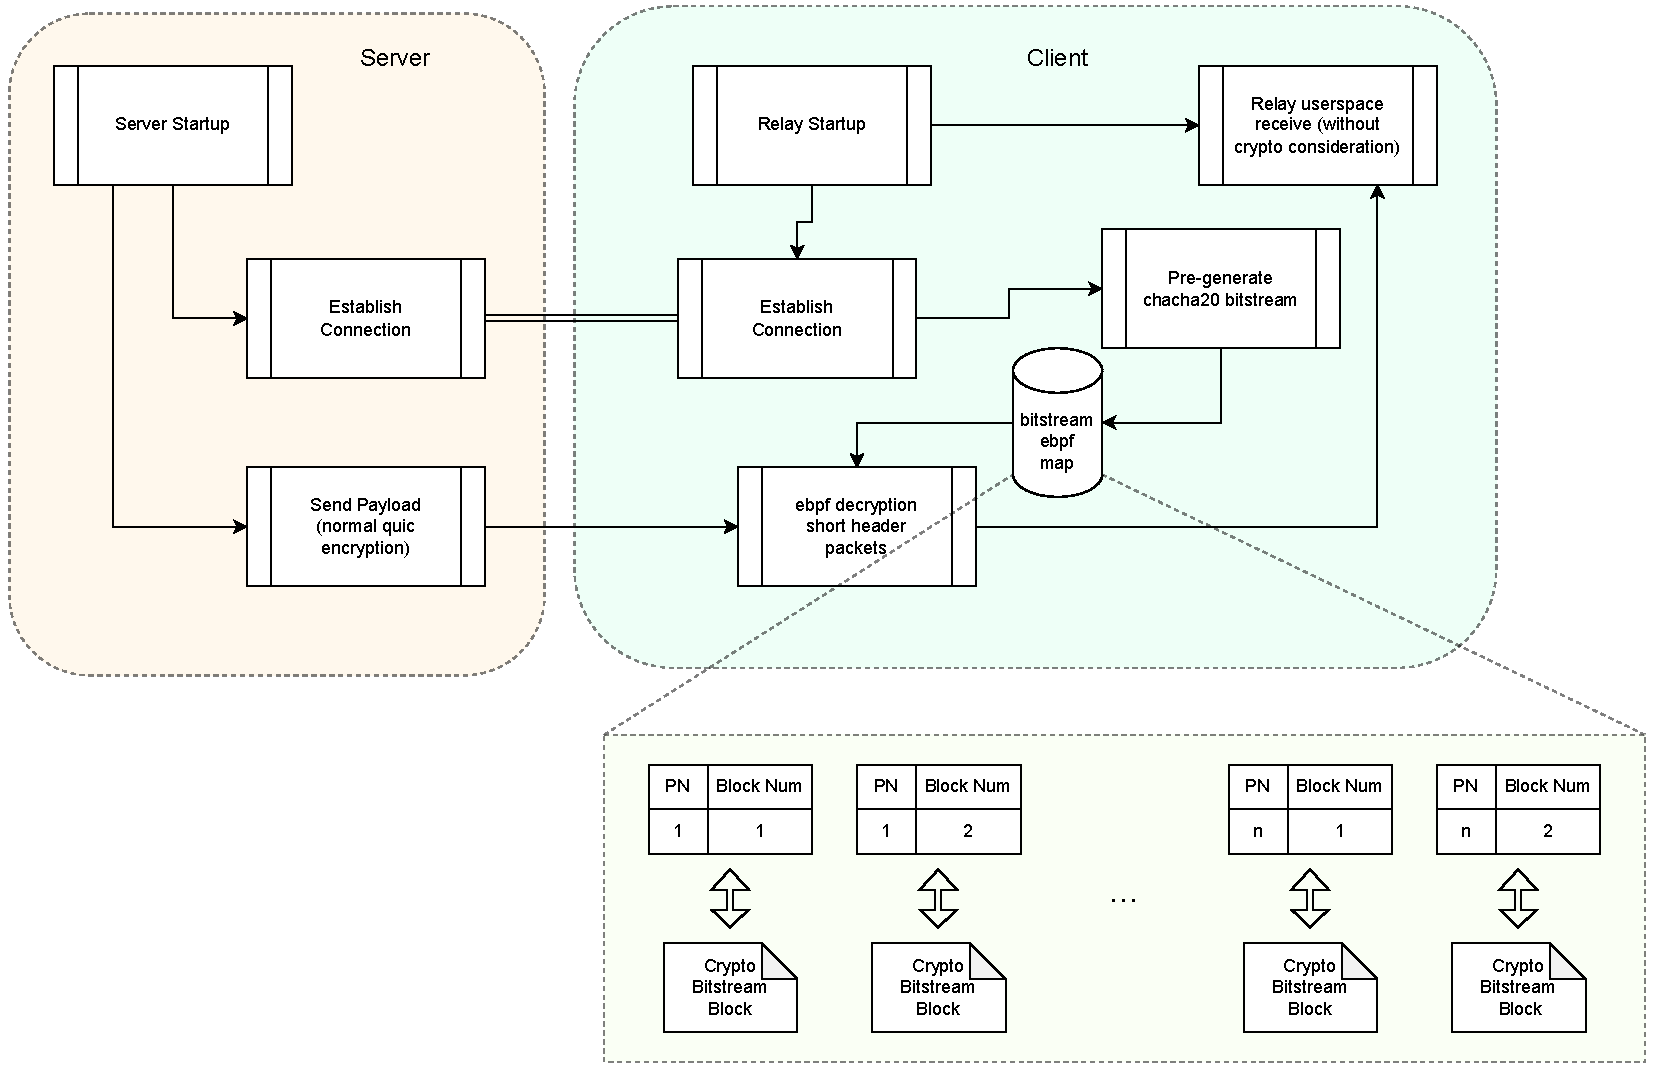
\includegraphics[width=\textwidth]{crypto_poc_interaction.pdf}
    \caption{Visual representation of the eBPF decryption setup}
    \label{fig:ebpf-crypto-setup}
\end{figure}

\vspace{2cm}

% TODO: create graphic on how the pre-generation looks and how it should work going forward when the data transfer already started

\section{Results}
Our proof of concept shows an example setup where a server sends an encrypted packet to a client, where it is decrypted by an eBPF program 
hooked to the TC subsystem.
In this simple initial implementation we omit some parts which are not immediately necessary for a first proof of concept.
For example we only consider packet decryption since encryption works the same way, we do not consider header en- and decryption, 
which are part of the QUIC protocol (those can be added later which should not pose an issue since the header encryption 
is also based on TLS 1.3 so all the used techniques already mentioned can be applied here as well. The computation effort is also small enough 
for an eBPF implementation.), the tag authentification has not yet been considered for simplicity and there support of all other cipher suites 
mentioned by TLS 1.3 is not yet given.
The last restriction is likely not as problematic as it sounds because despite the other suites of TLS 1.3 being based on block ciphers (AES-GCM and AES-CCM),
they behave similar to a stream cipher if we, on a high level, ignore the block-wise processing.
That should allow us to use similar approaches for AES-GCM and AES-CCM as we used for ChaCha20 even though it might have a few separate quirks
that need to be considered.
The proof of concept is also not yet integrated into the eBPF Fast-Relay setup of our previous work, but given that it is disjoint from the 
functionality of the other eBPF programs, this should not pose a problem.
For now what looks to be the biggest challenge for the full integration is an efficient way of handling the authentification tag of a packet.
The problem here is that the Poly1305 tag is dependent on the payload so pre-computing will not work.
One way to handle that would be to calculate the expected tag in the eBPF program itself and compare it to the tag in the packet.
This would be ideal and should be feasible within eBPF verify limits.
An alternative would be to let the userspace of the relay handle the tag verification but this might lead to the need for retroactive cancellation of packets
which is not ideal and might introduce additional problems like security vulnerabilities.

\section{Next Steps}
In order for our setup to be fully TLS 1.3 compliant, since TLS 1.3 does not allow the user to manually select one of the allowed ciphersuites, 
we would need to add support for all other ciphersuites that are potentially used in the protocol.
This would mean implementing AES-GCM and AES-CCM support for eBPF en- and decryption. 
As already mentioned, despite them being block ciphers a similar approach should be applicable.
Next steps would include this but probably have a focus on the authentification tag handling since this is the most critical part left for a full
support of the ChaCha20-Poly1305 cipher suite.

\section{References}
\printbibliography{}

\end{document}